% !TEX encoding = UTF-8 Unicode
\documentclass[a4paper]{article}

\usepackage{color}
\usepackage{url}
\usepackage[T2A]{fontenc} % enable Cyrillic fonts
\usepackage[utf8]{inputenc} % make weird characters work
\usepackage{graphicx}

\usepackage[english,serbian]{babel}
%\usepackage[english,serbianc]{babel} %ukljuciti babel sa ovim opcijama, umesto gornjim, ukoliko se koristi cirilica

\usepackage[unicode]{hyperref}
\hypersetup{colorlinks,citecolor=green,filecolor=green,linkcolor=blue,urlcolor=blue}

\usepackage{listings}

%\newtheorem{primer}{Пример}[section] %ćirilični primer
\newtheorem{primer}{Primer}[section]

\definecolor{mygreen}{rgb}{0,0.6,0}
\definecolor{mygray}{rgb}{0.5,0.5,0.5}
\definecolor{mymauve}{rgb}{0.58,0,0.82}

\lstset{ 
  backgroundcolor=\color{white},   % choose the background color; you must add \usepackage{color} or \usepackage{xcolor}; should come as last argument
  basicstyle=\scriptsize\ttfamily,        % the size of the fonts that are used for the code
  breakatwhitespace=false,         % sets if automatic breaks should only happen at whitespace
  breaklines=true,                 % sets automatic line breaking
  captionpos=b,                    % sets the caption-position to bottom
  commentstyle=\color{mygreen},    % comment style
  deletekeywords={...},            % if you want to delete keywords from the given language
  escapeinside={\%*}{*)},          % if you want to add LaTeX within your code
  extendedchars=true,              % lets you use non-ASCII characters; for 8-bits encodings only, does not work with UTF-8
  firstnumber=1000,                % start line enumeration with line 1000
  frame=single,	                   % adds a frame around the code
  keepspaces=true,                 % keeps spaces in text, useful for keeping indentation of code (possibly needs columns=flexible)
  keywordstyle=\color{blue},       % keyword style
  language=Python,                 % the language of the code
  morekeywords={*,...},            % if you want to add more keywords to the set
  numbers=left,                    % where to put the line-numbers; possible values are (none, left, right)
  numbersep=5pt,                   % how far the line-numbers are from the code
  numberstyle=\tiny\color{mygray}, % the style that is used for the line-numbers
  rulecolor=\color{black},         % if not set, the frame-color may be changed on line-breaks within not-black text (e.g. comments (green here))
  showspaces=false,                % show spaces everywhere adding particular underscores; it overrides 'showstringspaces'
  showstringspaces=false,          % underline spaces within strings only
  showtabs=false,                  % show tabs within strings adding particular underscores
  stepnumber=2,                    % the step between two line-numbers. If it's 1, each line will be numbered
  stringstyle=\color{mymauve},     % string literal style
  tabsize=2,	                   % sets default tabsize to 2 spaces
  title=\lstname                   % show the filename of files included with \lstinputlisting; also try caption instead of title
}

\begin{document}

\title{Šta čini univerzitetski kurs teškim?\\ \small{Seminarski rad u okviru kursa\\Metodologija stručnog i naučnog rada\\ Matematički fakultet}}

\author{Jovan Vukićević, Jovan Škorić, Nikola Kuburović, Radenko Nikolić\\ jovanvukicevic@hotmail.com, email drugog, trećeg, četvrtog autora}

%\date{9.~april 2015.}

\maketitle

\abstract{
Teški univerzitetski kursevi predstavljaju jednu od glavnih prepreka pri studentovom prolasku kroz studije. U ovom radu istražujemo različite faktore organizacije kurseva koji utiču na njihovu težinu, počev od aspekata organizacije nastave do aspekata organizacije ispita. Na kraju rada prikazujemo rezultate ankete sprovedene nad studentima Matematičkog fakulteta Univerziteta u Beogradu i predstavljamo njihova lična iskustva sa teškim univerzitetskim kursevima, kao i upoređujemo dobijene zaključke sa zaključcima u literaturi.
}

\tableofcontents

\newpage

\section{Uvod}
\label{sec:uvod}

Srž studija na univerzitetu čine univerzitetski kursevi. Samim tim, težinu studija možemo poistovetiti sa težinom kurseva na njima. Iako se u osnovi težine univerzitetskog kursa nalaze kompleksnost same oblasti koja se obrađuje i količina studentskog predznanja, postoje razni drugi faktori koji doprinose težini kursa.

Glavni cilj univerzitetskih profesora je da prenesu znanje studentima na što efikasniji način, što podrazumeva jednostavnost u prenošenju iskustava u razumevanju problema. U odnosu na nastavnike na prethodnim obrazovnim nivoima, univerzitetski profesori imaju mnogo veću slobodu u dizajniranju kurseva koje predaju. Podešavanjem raznih aspekata tih kurseva, oni direktno utiču na njegovu težinu.

Kao pomoć profesorima u dizajniranju svojih kurseva, kao i uvid u šta to čini univerzitetski kurs teškim, u ovom radu ćemo prikazati osnovne karakteristike teških univerzitetskih kurseva, kao i dati predloge kako ih načiniti lakšim. Zarad ovog cilja, sproveli smo i anketu nad studentima Matematičkog fakulteta Univerziteta u Beogradu, čiji rezultat ćemo prezentovati u ovom radu.

\section{Ogranizacija nastave}
Organizacija nastave ima ključnu ulogu u oblikovanju univerzitetskog iskustva studenata i
značajno utiče na percepciju težine kursa. Na osnovu dostupne literature, nekoliko ključnih
faktora doprinosi efektivnoj organizaciji nastave: jasno definisani ishodi učenja, pažljivo
strukturisanje sadržaja, odgovarajući tempo predavanja i primena praktičnih primera u
nastavi.

\subsection{Ishodi učenja i planiranje nastave}
Jasno definisani ishodi učenja čine osnovu uspešne organizacije nastave. Ishodi moraju biti
usklađeni s industrijskim standardima i realnim potrebama tržišta rada kako bi studenti mogli
da povežu teorijsko znanje sa praktičnim zahtevima profesije. Teorija konstruktivne
usklađenosti (slika \ref{fig:konstruktivna_uskladjenost}), koju su predložili Biggs i Tang (2007), naglašava da ishodi učenja, nastavne
aktivnosti i ocenjivanje treba da budu međusobno povezani kako bi se maksimizovala
efikasnost obrazovnog procesa. Ova usklađenost ne samo da poboljšava razumevanje, već i
smanjuje osećaj zbunjenosti kod studenata, što direktno utiče na percepciju težine kursa.

Literatura takođe ističe potrebu za dubinskim pokrivanjem osnovnih koncepata, umesto
pokušaja da se obuhvati širok spektar tema bez dovoljno objašnjenja. Kane, Rockoff i
Staiger (2006) navode da prevelika količina gradiva, koja nije jasno povezana s praktičnim
primerima, često dovodi do pada akademskih postignuća studenata. Slično tome, Smith
(2009) ističe da neuspeh u naglašavanju osnovnih veština i znanja utiče na percepciju kursa
kao teškog. Osnovno pravilo je da kurikulum treba da bude prilagođen razumevanju
studenata, s progresivnim uvodom u složenije teme kako bi se omogućio postepen prelazak
na naprednije koncepte.

Učestali problemi s organizacijom nastave uključuju uključivanje suvišnih ili nepotrebnih
tema u kurikulum, nedostatak jasnoće u vezi sa sekvenciranjem gradiva i neprilagođeno
vreme za pojedine teme. Na primer, istraživanja su pokazala da neadekvatno vremensko
planiranje za pojedine aspekte gradiva često dovodi do osećaja preopterećenja kod
studenata.

\begin{figure}[h!]
\begin{center}
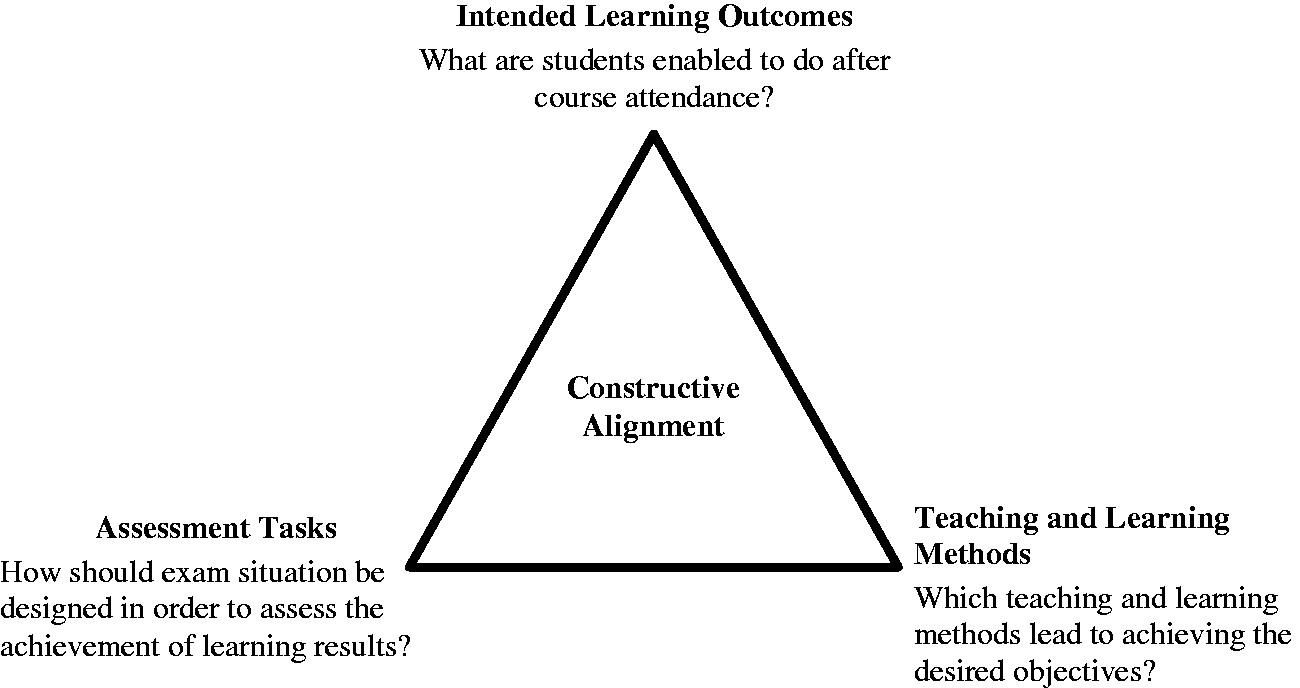
\includegraphics[scale=2]{constructive_alignment.jpeg}
\end{center}
\caption{Konstruktivna usklađenost}
\label{fig:konstruktivna_uskladjenost}
\end{figure}

\subsection{Tempo izvođenja nastave}
Tempo nastave značajno utiče na percepciju težine kursa i na sposobnost studenata da
razumeju i savladaju gradivo. Brza predavanja, koja ne ostavljaju prostor za diskusiju i
dodatna objašnjenja, mogu povećati osećaj frustracije kod studenata. Prema istraživanjima,
loše tempirana nastava često ostavlja studente s nedovoljno vremena za procesuiranje
informacija, što negativno utiče na rezultate ispita i percepciju kursa.

Daka (2019) navodi da je pažljivo planiranje nastavnih aktivnosti ključno za uspešnu
nastavu. Uključivanje raznovrsnih nastavnih metoda, kao što su praktične vežbe, grupni rad i
studije slučaja, doprinosi dubljem razumevanju gradiva i povećava angažovanost studenata.
Changwe i saradnici (2023) sugerišu da predavači treba da izbegavaju prebrzo prelazak s
jedne teme na drugu, jer to može izazvati zbunjenost i otežati praćenje nastave
Još jedan važan aspekt tempa nastave je korišćenje jasno definisanih prelaza između
različitih delova predavanja. Na primer, jasno razdvajanje tema i objašnjenja omogućava
studentima da prepoznaju ključne tačke predavanja, što dodatno pomaže u zadržavanju
pažnje i razumevanju kompleksnih tema. Pored toga, postavljanje logičnog toka gradiva, gde
se složene teme nadovezuju na osnovne koncepte, značajno doprinosi smanjenju osećaja
preopterećenja.

\subsection{Relevantnost sadržaja}
Sadržaj kursa mora biti jasno povezan sa stvarnim aplikacijama i profesionalnim zahtevima,
jer to povećava motivaciju i angažovanost studenata. Predavanja koja uspešno povezuju
teorijske koncepte s praktičnim primerima omogućavaju studentima da bolje razumeju kako
se stečeno znanje primenjuje u praksi. Sarfraz i saradnici (2022) navode da je kombinacija
tradicionalne nastave i tehnologije, kao što je kombinovano učenje (eng.~{\em blended learning}, slika \ref{fig:kombinovano_ucenje}), posebno korisna za studente
jer omogućava fleksibilniji pristup učenju i bolju primenu gradiva.

Problemi nastaju kada kursevi sadrže previše zastarelih ili nerelevantnih tema. Na primer,
ako predavanja uključuju koncepte koji više nisu primenljivi u modernim profesionalnim
okruženjima, studenti gube interes i kurs se doživljava kao suvišno težak. Na osnovu
istraživanja, prilagođavanje sadržaja savremenim industrijskim standardima i kontinuirano
preispitivanje kurikuluma ključno je za rešavanje ovih problema.

\begin{figure}[h!]
\begin{center}
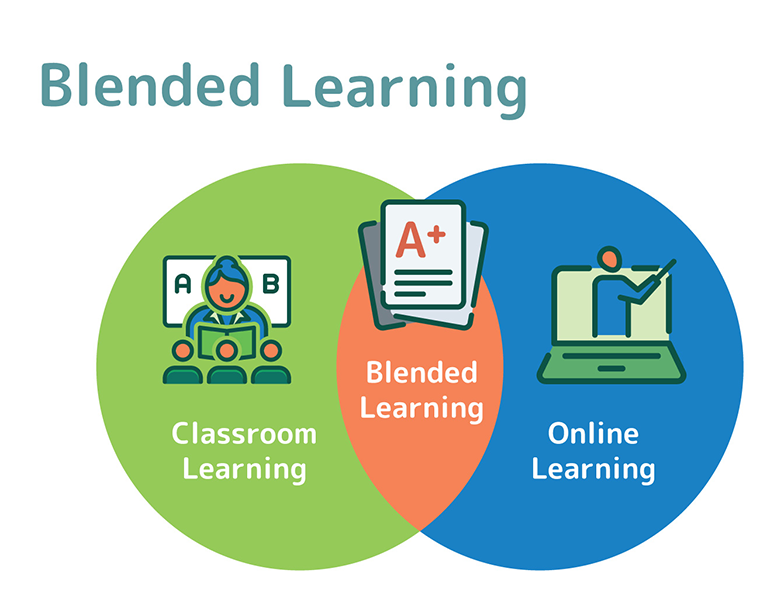
\includegraphics[scale=0.4]{blended_learning.png}
\end{center}
\caption{Kombinovano učenje}
\label{fig:kombinovano_ucenje}
\end{figure}

Ovi elementi organizacije nastave ključni su za oblikovanje akademskog iskustva studenata.
Pažljivo osmišljeni kursevi, sa jasno definisanim ciljevima i odgovarajućim tempom, ne samo
da smanjuju percepciju težine kursa, već i obezbeđuju kvalitetnije obrazovanje i bolje
rezultate.

\section{Engleski termini i citiranje}	
\label{sec:termini_i_citiranje}

Na svakom mestu u tekstu naglasiti odakle tačno potiču informacije. Uz sve novouvedene termine u zagradi naglasiti od koje engleske reči termin potiče. 

Naredni primeri ilustruju način uvođenja enlegskih termina kao i citiranje.

\begin{primer}
Problem zaustavljanja (eng.~{\em halting problem}) je neodlučiv \cite{haltingproblem}.
\end{primer}

\begin{primer}
Za prevođenje programa napisanih u programskom jeziku C može se koristiti GCC kompajler \cite{gcc}.
\end{primer}

\begin{primer}
 Da bi se ispitivala ispravost softvera, najpre je potrebno precizno definisati njegovo ponašanje \cite{laski2009software}. 
\end{primer}

Reference koje se koriste u ovom tekstu zadate su u datoteci {\em seminarski.bib}. Prevođenje u pdf format u Linux okruženju može se uraditi na sledeći način:
\begin{verbatim}
pdflatex TemaImePrezime.tex 
bibtex TemaImePrezime.aux 
pdflatex TemaImePrezime.tex 
pdflatex TemaImePrezime.tex 
\end{verbatim}
Prvo latexovanje je neophodno da bi se generisao {\em .aux} fajl. {\em bibtex} proizvodi odgovarajući {\em .bbl} fajl koji se koristi za generisanje literature. 
Potrebna su dva prolaza (dva puta pdflatex) da bi se reference ubacile u tekst (tj da ne bi ostali znakovi pitanja umesto referenci). Dodavanjem novih referenci potrebno je ponoviti ceo postupak.  











Broj naslova i podnaslova je proizvoljan. Neophodni su samo Uvod i Zaključak. Na poglavlja unutar teksta referisati se po potrebi. 
\begin{primer}
U odeljku \ref{sec:naslov1} precizirani su osnovni pojmovi, dok su zaključci dati u odeljku \ref{sec:zakljucak}.
\end{primer}

Još jednom da napomenem da nema razloga da pišete:
\begin{verbatim}
\v{s} i \v{c} i \'c ...
\end{verbatim}
Možete koristiti srpska slova
\begin{verbatim}
š i č i ć ... 
\end{verbatim}



\section{Slike i tabele}
\label{slike_i_tabele}

Slike i tabele treba da budu u svom okruženju, sa odgovarajućim naslovima, obeležene labelom da koje omogućava referenciranje. 

\begin{primer} Ovako se ubacuje slika. Obratiti pažnju da je dodato i 
\begin{verbatim}
\usepackage{graphicx}
\end{verbatim}

\begin{figure}[h!]
\begin{center}
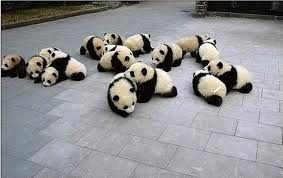
\includegraphics[scale=0.75]{panda.jpg}
\end{center}
\caption{Pande}
\label{fig:pande}
\end{figure}

Na svaku sliku neophodno je referisati se negde u tekstu. Na primer, na slici \ref{fig:pande} prikazane su pande. 
\end{primer}

\begin{primer} I tabele treba da budu u svom okruženju, i na njih je neophodno referisati se u tekstu. Na primer, u tabeli \ref{tab:tabela1} su prikazana različita poravnanja u tabelama.

\begin{table}[h!]
\begin{center}
\caption{Razlčita poravnanja u okviru iste tabele ne treba koristiti jer su nepregledna.}
\begin{tabular}{|c|l|r|} \hline
centralno poravnanje& levo poravnanje& desno poravnanje\\ \hline
a &b&c\\ \hline
d &e&f\\ \hline
\end{tabular}
\label{tab:tabela1}
\end{center}
\end{table}

\end{primer}

\section{K\^{o}d i paket listings}
Za ubacivanje koda koristite paket \textbf{listings}:
\url{https://en.wikibooks.org/wiki/LaTeX/Source_Code_Listings}

\begin{primer}
Primer ubacivanja koda za programski jezik Python dat je kroz listing \ref{simple}. Za neki drugi programski jezik, treba podesiti odgvarajući programski jezik u okviru defnisanja stila.
\end{primer}
\begin{lstlisting}[caption={Primer ubacivanja koda u tekst},frame=single, label=simple]
# This program adds up integers in the command line
import sys
try:
    total = sum(int(arg) for arg in sys.argv[1:])
    print 'sum =', total
except ValueError:
    print 'Please supply integer arguments'
\end{lstlisting}


\section{Prvi naslov}
\label{sec:naslov1}


Ovde pišem tekst. 
Ovde pišem tekst. 
Ovde pišem tekst. 
Ovde pišem tekst. 
Ovde pišem tekst. 
Ovde pišem tekst. 
Ovde pišem tekst. 
Ovde pišem tekst. 


\subsection{Prvi podnaslov}
\label{subsec:podnaslov1}

Ovde pišem tekst. 
Ovde pišem tekst. 
Ovde pišem tekst. 
Ovde pišem tekst. 
Ovde pišem tekst. 
Ovde pišem tekst. 
Ovde pišem tekst. 

\subsection{Drugi podnaslov}
\label{subsec:podnaslov2}

Ovde pišem tekst. 
Ovde pišem tekst. 
Ovde pišem tekst. 
Ovde pišem tekst. 
Ovde pišem tekst. 
Ovde pišem tekst. 


\subsection{... podnaslov}
\label{subsec:podnaslovN}

Ovde pišem tekst. 
Ovde pišem tekst. 
Ovde pišem tekst. 
Ovde pišem tekst. 
Ovde pišem tekst. 
Ovde pišem tekst. 

\section{n-ti naslov}
\label{sec:naslovN}

Ovde pišem tekst. 
Ovde pišem tekst. 
Ovde pišem tekst. 
Ovde pišem tekst. 
Ovde pišem tekst. 

\subsection{... podnaslov}
\label{subsec:podnaslovK}

Ovde pišem tekst. 
Ovde pišem tekst. 
Ovde pišem tekst. 
Ovde pišem tekst. 
Ovde pišem tekst. 

\subsection{... podnaslov}
\label{subsec:podnaslovM}

Ovde pišem tekst. 
Ovde pišem tekst. 
Ovde pišem tekst. 
Ovde pišem tekst. 
Ovde pišem tekst. 


\section{Zaključak}
\label{sec:zakljucak}

Težina univerzitetskih kurseva predstavlja veoma bitan aspekt studentskog akademskog iskustva. Univerzitet treba da bude mesto gde studenti, osim što se edukuju za odabranu oblast, imaju lični napredak i spremaju se za buduće izazove. Neadekvatna težina univerzitetskih kurseva negativno utiče na ove ciljeve, a samim tim, i na budući uspeh, ne samo u akademiji, nego i životu studenata. 

U ovom radu smo predstavili najosnovnije karakteristike teških univerzitetskih kurseva. Počev od aspekata vezanih za organizaciju nastave zaključili smo da neadekvatni nastavni materijali, materijali niskog kvaliteta ili materijali nerelevantni za današnje vreme, znatno doprinose težini kursa. Studentu koji nema motivaciju da uči, ili nema odakle da uči o određenoj oblasti, će kurs teže pasti nego studentu koji poseduje ove osobine. Takođe, zaključili smo da je način održavanja nastave, kroz tempo predavanja i interakciju predavača sa studentima, od ključnog značaja za studentovu percepciju težine kursa. Predavanja prevelike brzine mogu dovesti do nerazumevanja gradiva, a samim tim, i do kasnijeg otežavanja učenja istog, dok prespora ili neinteraktivna predavanja mogu biti dosadna i doprinose padu motivacije i koncentracije studenta. Obradili smo i karakteristike ispita koje doprinose težini kursa i zaključili da aspekti kao što su prevelika modularnost i nepovezanost između tih modula, loša korelacija između težine ispita i težine materijala kursa, kao i nenadoknadive provere znanja pre samog ispita direktno otežavaju kurs.

Sprovođenjem ankete nad studentima Matematičkog fakulteta Univerziteta u Beogradu, saznali smo za koje aspekte univerzitetskih kurseva oni smatraju da najviše doprinose težini istog. Prikazali smo rezultate ankete i uporedili ih sa zaključcima u relevantnoj literaturi.

\addcontentsline{toc}{section}{Literatura}
\appendix
\bibliography{seminarski} 
\bibliographystyle{plain}

\appendix
\section{Dodatak}
Ovde pišem dodatne stvari, ukoliko za time ima potrebe.
Ovde pišem dodatne stvari, ukoliko za time ima potrebe.
Ovde pišem dodatne stvari, ukoliko za time ima potrebe.
Ovde pišem dodatne stvari, ukoliko za time ima potrebe.
Ovde pišem dodatne stvari, ukoliko za time ima potrebe.


\end{document}
